\documentclass[5p]{elsarticle}
%\documentclass[review]{elsarticle}

\usepackage{lineno,hyperref}
\modulolinenumbers[5]

\journal{Journal of Hydrology}


\usepackage{multirow}
\usepackage{gensymb}
\usepackage{subcaption}
%\usepackage{amsmath}


%%%%%%%%%%%%%%%%%%%%%%%
%% Elsevier bibliography styles
%%%%%%%%%%%%%%%%%%%%%%%
%% To change the style, put a % in front of the second line of the current style and
%% remove the % from the second line of the style you would like to use.
%%%%%%%%%%%%%%%%%%%%%%%

%% Numbered
%\bibliographystyle{model1-num-names}

%% Numbered without titles
%\bibliographystyle{model1a-num-names}

%% Harvard
\bibliographystyle{model2-names}\biboptions{authoryear}

%% Vancouver numbered
%\usepackage{numcompress}\bibliographystyle{model3-num-names}

%% Vancouver name/year
%\usepackage{numcompress}\bibliographystyle{model4-names}\biboptions{authoryear}

%% APA style
%\bibliographystyle{model5-names}\biboptions{authoryear}

%% AMA style
%\usepackage{numcompress}\bibliographystyle{model6-num-names}

%% `Elsevier LaTeX' style
%\bibliographystyle{elsarticle-num}
%%%%%%%%%%%%%%%%%%%%%%%

\begin{document}

\begin{frontmatter}

\title{Using Genetic Algorithms to Optimize the Analogue Method for Precipitation Forecasting in the Swiss Alps}

%% Group authors per affiliation:
\author[unil,terranum]{Pascal Horton\corref{mycorrespondingauthor}}
\cortext[mycorrespondingauthor]{Corresponding author}
\ead{pascal.horton@alumnil.unil.ch}

\author[unil]{Michel Jaboyedoff}
\author[lthe]{Charles Obled}

\address[unil]{University of Lausanne, Lausanne, Switzerland}
\address[terranum]{Terranum LLC, Rue de l'industrie 35 bis, 1030 Bussigny, Switzerland}
\address[lthe]{Universit\'{e} de Grenoble-Alpes, LTHE, Grenoble, France}

\begin{abstract}
The analogue method is often used to forecast precipitation based on predictors variables provided by global models. The method samples a selection of days in the archives that are similar to the target day to forecast, and consider the corresponding observed precipitation (the predictand) as the conditional distribution for the target day. The statistical relationship between predictors and predictands relies on some parameters that characterize how and where the similitude between two atmospheric situations has to be defined.

This relationship is usually established by a semi-automatic sequential procedure that has strong limitations. A new global optimization approach relying on Genetic Algorithms can optimize all parameters jointly and automatically, which is a breakthrough in the way the analogue method was calibrated until now. It allows taking into account parameters inter-dependencies, adding new degrees of freedom, and choosing objectively some parameters that were manually selected beforehand (such as the pressure levels and the temporal windows of the predictor variables).

In this work, the global optimization is applied to the Rh\^{o}e catchment in the Swiss Alps in order to show its interest and the relevance of the resulting parameters. Indeed, not only the performance increases, but the parameters are obtained automatically and objectively, which reduces effort-hours when adapting the method to a new region or for a new predictand. Moreover, the approach allows for new degrees of freedom, such as a weighting between the pressure levels and non overlapping spatial windows.
\end{abstract}

\begin{keyword}
Precipitation\sep
Analogue method\sep
Optimization\sep
Genetic algorithms\sep
Alpine climate
\end{keyword}

\end{frontmatter}

\linenumbers

\section{Introduction}
\label{sec:intro}

The analogue method (AM) is a downscaling technique based on the idea expressed by \citet{Lorenz1956, Lorenz1969}, that similar situations in terms of atmospheric circulation are likely to lead to similar local weather \citep{Duband1970, Bontron2005}. It aims at forecasting a predictand, often the daily precipitation \citep[eg.]{Guilbaud1997, Bontron2005, Bliefernicht2010, Marty2012, Horton2012, Radanovics2013, BenDaoud2015}, on the basis of predictor variables describing the synoptic atmospheric circulation. Other predictands are also often considered \citep[see][for a non-exhaustive list]{Horton2016}.

In operational forecasting, it has been used mainly by practitioners, notably hydropower companies or flood forecasting services, while in climate studies, it is newly used to downscale the results of global climate model (GCM) simulation runs. In this last case, although the GCM represents the large or regional scale evolutions of the atmosphere, it would be far too computer intensive to get down to variables such as precipitation at a rather small and representative scale. Therefore the idea to rely on past observations to bypass these unaffordable small scale simulations and to go from the large scale situation proposed by the GCM to the end variables like precipitation by searching anlogs in the past and present archive. 

The method can be made of multiple successive subsampling steps, each of them relying on different meteorological variables. A certain number of parameters define the relationship between predictors and predictands, such as the choice of the predictor variable, its pressure level and temporal window to consider, the spatial domain to use for the comparison, as well as the analogy criteria itself, and finally the number of analogue situations to keep at each subsampling level. These parameters are usually calibrated by means of a semi-automatic sequential procedure \citep[see][for the details]{Bontron2004, Horton2016}. This sequential approach has strong limitations: (i) it cannot automatically choose the pressure levels and the temporal windows for a given meteorological variable, (ii) it cannot handle dependencies between the parameters within a level of analogy, and even less between them, and (iii) it could not handle new degrees of freedom, such as a weighting between the pressure levels. Thus, even if the processing involved is relatively fast, the sequential approach requires laborious assessments of predictors combinations (variables, pressure levels, temporal windows), and present a high risk of ending in a local optimum due to subjective initial choices and lack of consideration of parameters dependencies.

With the perspective to overcome these limitations, a global optimization technique, namely Genetic Algorithms (GAs) was introduced by \citet{Horton2016a}. An intensive assessment work resulted in recommendations of parametrization of GAs in order to optimize AMs successfully. The present paper is based on these recommendations and apply them to precipitation forecasting for the upper Rh\^{o}e catchment in the Swiss Alps. It aims at proving the relevance of a fully-automatic, objective, and global, optimization technique for AMs. The applications are indeed numerous, as the AM has to be adapted to every new location it is applied, or to any new predictand it should forecast.

A short overview of AMs is presented in section \ref{sec:analog_method}, as well as a summary of Genetic Algorithms in section \ref{sec:gas}. Section \ref{sec:case_study} describes the case study area. The results are first detailed for the optimization of the analogy on the atmospheric circulation only (section \ref{sec:optim_circul}), before being extended to a method adding a second level of analogy on moisture variables (section \ref{sec:optim_moisture}). General discussions (section \ref{sec:discussion}) and conclusions (section \ref{sec:conclusions}) follow.


\section{The analogue method}
\label{sec:analog_method}

\subsection{References}
\label{sec:references}

Multiple variations of the methods exist, and most of them will not be detailed hereafter \cite[see][for more comprehensive listings]{Horton2016, BenDaoud2015}. However, there are mainly 2 parametrizations that are most often used for precipitation forecasting and that will be considered as reference: one that relies on an analogy of the atmospheric circulation, and another that adds a second level of analogy on moisture variables \citep{Obled2002, Bontron2005, Marty2012}.

The method based on the analogy of the synoptic circulation consists in the following steps (Table \ref{table:params_R1}): the similarity of the atmospheric circulation of a target date with every day of the archive is assessed by processing the S1 criteria \citep[Eq.\ (\ref{eq:S1}), ][]{Teweles1954, Drosdowsky2003}, which is a comparison of gradients, over a certain spatial window. \citet{Bontron2005} showed that the geopotential height at 500~hPa and 1000~hPa are the best first predictors of the NCEP/NCAR reanalysis dataset, and that the S1 criteria performs better than scores based on absolute distances. The reason for such better results is that the S1 criteria allows comparing the circulation pattern, by means of the gradients, rather than the absolute value of the geopotential height. To cope with seasonal effects, candidate dates are extracted within a period of 4 months centred around the target date, for every year of the archive. Following the nomenclature proposed by \citet{Horton2016}, this method will be named 2Z.

\begin{equation}
\label{eq:S1}
S1=100 \frac {\displaystyle \sum_{i} \vert \Delta\hat{z}_{i} - \Delta z_{i} \vert}
{\displaystyle \sum_{i} max\left\lbrace \vert \Delta\hat{z}_{i} \vert , \vert \Delta z_{i} \vert \right\rbrace }
\end{equation}
where $\Delta \hat{z}_{i}$ is the forecast geopotential height difference between the \textit{i}th pair of adjacent points of the gridded data describing the target situation, and $\Delta z_{i}$ is the corresponding observed geopotential height difference in the candidate situation. The differences are processed separately in both directions. The smaller the S1 values are, the more similar the pressure fields.

\begin{table}[htbp]
	\caption{Parameters of the reference method on the atmospheric circulation (2Z).}
	\footnotesize
	\begin{center}
		\begin{tabular}{ccccc}
			\hline
			Level & Variable & Hour & Criteria & Nb \\ 
			\hline 
			0 & \multicolumn{4}{l}{$\pm 60$ days around the target date} \\
			\hline 
			\multirow{2}{*}{1} & Z 1000~hPa & 12~h & \multirow{2}{*}{S1} & \multirow{2}{*}{50} \\
			& Z 500~hPa & 24~h & & \\ 
			\hline 
		\end{tabular} 
	\end{center}
	\label{table:params_R1}
\end{table}

The $N_{1}$ dates with the lowest values of S1 are considered as analogues to the target day. The number of analogues, $N_{1}$, is a parameter to calibrate. Then, the daily observed precipitation amount of the $N_{1}$ resulting dates provide the empirical conditional distribution considered as the probabilistic forecast for the target day.

The other most know parametrization adds a second level of analogy on moisture variables (method 2Z-2MI, Table \ref{table:params_R2}). The predictor that \citet{Bontron2004} found optimal for the France territory is a moisture index made of the product of the precipitable water with the relative humidity at 850~hPa. \cite{Horton2012a} confirmed that this index is better for the Swiss Alps than any other variable from the NCEP/NCAR reanalysis considered independently. When adding a second level of analogy, we subsample $N_{2}$ dates in the $N_{1}$ analogues on the atmospheric circulation, to end up with a smaller number of analogue situations. When we add a second level of analogy, we keep a higher number of analogues on the first level.

\begin{table}[htbp]
	\caption{Parameters of the reference method with moisture variables (2Z-2MI).}
	\footnotesize
	\begin{center}
		\begin{tabular}{ccccc}
			\hline 
			Level & Variable & Hour & Criteria & Nb \\ 
			\hline 
			0 & \multicolumn{4}{l}{$\pm 60$ days around the target date} \\
			\hline 
			\multirow{2}{*}{1} & Z 1000~hPa & 12~h & \multirow{2}{*}{S1} & \multirow{2}{*}{70} \\
			& Z 500~hPa & 24~h & & \\ 
			\hline
			\multirow{2}{*}{2} & TPW * RH 850~hPa & 12~h & \multirow{2}{*}{RMSE} & \multirow{2}{*}{30} \\
			& TPW * RH 850~hPa & 24~h & & \\ 
			\hline 
		\end{tabular} 
	\end{center}
	\label{table:params_R2}
\end{table}


\subsection{Data}
\label{sec:data}

The AM relies on two types of data: predictors, that are atmospheric variables describing the state of the atmosphere at a synoptic scale, and the predictand, which is the local weather time series we want to forecast.

Predictors are generally reanalysis datasets. NCEP-NCAR reanalysis \citep[6-hourly, 17 pressure levels at a resolution of 2.5\degree, see][]{Kalnay1996} are used here, but it can be any other reanalysis dataset.

The predictand (which is to be predicted) is in here the daily precipitation (6~a.m. to 6~a.m. the next day) measured at the MeteoSwiss' stations network, for the period 1961-2008. The time series from every available gauging station were averaged over subregions in order to smooth local effects \citep{Obled2002, Marty2012}.


\subsection{Performance assessment}
\label{sec:score}

The most used score to assess an AM performance is the CRPS \citep[Continuous Ranked Probability Score,][]{Brown1974, Matheson1976, Hersbach2000}. It allows assessing the predicted cumulative distribution functions $F(y)$, for example of the precipitation values $y$ from analogue situations, compared to the observed value $y^{0}$. The better the forecast, the smaller the score. The mean CRPS of a forecast series of length $n$ can be written:

\begin{equation}
\label{eq:CRPS}
CRPS = \frac{1}{n} \sum_{i=1}^{n} \left(  \int_{-\infty}^{+\infty} \left[ F_{i}(y)-H_{i}(y-y_{i}^{0})\right]^{2} dy \right) 
\end{equation}
where $H(y-y_{i}^{0})$ is the Heaviside function that is null when $y-y_{i}^{0}<0$, and has the value 1 otherwise. The mean CRPS is averaged on the calibration, respectively the validation periods, on all days.

This score is now commonly used for the evaluation of continuous variables prediction systems \citep{Casati2008, Marty2010}. To compare the value of the score in regard to a reference, we often consider its skill score value, and use the climatological distribution as the reference. The CRPSS (\textit{Continuous Ranked Probability Skill Score}) is thus defined as following:

\begin{equation}
\label{eq:CRPSS}
CRPSS = \frac{CRPS-CRPS_{r}}{CRPS_{p}-CRPS_{r}} = 1-\frac{CRPS}{CRPS_{r}}
\end{equation}
where $CRPS_{r}$ is the CRPS value for the reference and $CRPS_{p}$ would be the one for a perfect forecast (which implies $CRPS_{p}~=~0$). A better forecast is characterized by an increase in CRPSS.


\section{Genetic algorithms}
\label{sec:gas}

Genetic Algorithms (GAs) were developed by \citet{Holland1992b} and popularized by \citet{Goldberg1989}. They are part of evolutionary algorithms \citep{Back1993b, Schwefel1993}, which get inspiration from some mechanisms of biological evolution, such as reproduction, genetic mutations, chromosomal crossovers, and natural selection. GAs seek the global optimum on a complex surface, theoretically without restriction. Practically, GAs allow rapidly approaching satisfactory solutions, but they do not provide the optimum solution for sure \citep{Zitzler2004a}. It is indeed mainly a matter of time. When the optimizer gets closer to the global optimum, any new improvement takes more time to appear (see figure \ref{fig:evolution}), and the final adjustment of the parameters is very time consuming \citep{Back1993a}. For problems that require a significant amount of time in order to evaluate the objective function, as in our case, we have to limit the number of generations to get reasonable processing time. Thus, different acceptable solutions can result from one or more optimizations \citep{Holland1992b}. This is a strength and a weakness of GAs: they are very good at exploring complex parameter spaces in order to identify the most promising areas, but they will not necessarily find the best solution with the optimal values of all parameters \citep{Holland1992b}.

The optimizations were performed based on the recommended GAs parametrization for AMs as described in \citet{Horton2016a}. As the optimization is mostly sensitive to the mutation operator (that randomly changes some values in the parameters sets), we consider parallel optimizations with variants of this operator, according to \citet{Horton2016a}:

\begin{itemize}
	\item 3x non-uniform mutation \citep{Michalewicz1996} with varying parameters,
	\item 1x multi-scale mutation \citep{Horton2016a},
	\item 2x chromosome of adaptive search radius \citep{Horton2016a}
\end{itemize}

A population size of 500 individuals (parameters sets of the AM) was considered, and the optimization was stopped when the best individual (with the highest CRPSS performance score) did not evolve for 20 generations (cycles of the optimization).


\section{Case study description}
\label{sec:case_study}

The study area is the alpine upper Rh\^{o}ne catchment in Switzerland (Fig.\ \ref{fig:map}). The altitude ranges from 372 to 4634~m.a.s.l.\ and the area is 5524~km$^{2}$. This region is the target of the MINERVE (Mod\'{e}lisation des Intemp\'{e}ries de Nature Extr\^{e}me sur les Rivi\`{e}res Valaisannes et de leurs Effets) project that aims at providing a real-time flood management on the upper Rh\^{o}ne catchment \citep{GarciaHernandez2009b}. Even thought the region is rather small, the meteorological influences related to extreme weather conditions varies substantially within it \citep[see][]{Horton2012}. Based on different climatological analyses, the gauging stations in the catchment were clustered in 10~subregions (Fig.\ \ref{fig:map}) :

\begin{enumerate}
	\item Swiss Chablais
	\item Trient Valley
	\item West Bernese Alps
	\item Lower Rhone Valley
	\item Left side valleys
	\item Southern ridges
	\item Upper Rhone Valley
	\item Southeast ridges
	\item East Bernese Alps
	\item Conches Valley
\end{enumerate}

The 48 years precipitation dataset (see section \ref{sec:intro}.\ref{sec:data}) was divided into a calibration period (CP) and a validation period (VP). Using data independent from the CP to validate our results is very important in order to assess the robustness of the improvements and to avoid overparametrization of the method.

In order to reduce potential bias related to trends in the climate change or to the evolution in measurement techniques, the selection of the VP is evenly distributed over the entire series \citep{BenDaoud2010}. Thus, we selected one year every six years for validation, which represents a total of 8 years for the VP and 40 for CP. The choice of the sequence was made in order to have similar statistical characteristics between the CP and the VP.


\section{Optimization of the circulation analogy}
\label{sec:optim_circul}

We first optimized the analogy of atmospheric circulation alone, without moisture variables, for the 10 subregions. We started from the most simple AM, and increased the complexity in order to identify the degrees of freedom that are of particular interest. Thus, the tested parametrization evolved iteratively in complexity. We do not provide the detailed results of the intermediate stages \citep[see][for the details]{Horton2012a}, but only the main conclusions.

We first considered the reference method for the analogy of the atmospheric circulation (2Z, Table \ref{table:params_R1}), based on the 500 and 1000~hPa levels. We let the optimizer choose the number of analogues, both spatial windows with no overlapping constraint, as well as the temporal window (hours of observation of the geopotential), what the sequential calibration cannot do. With these degrees of freedom, we could gain a relative CRPSS improvement of 3.97\% and 2.45\% in average for the CP and the VP respectively. Some tests showed that most of the gains are due to the non-overlapping spatial windows. This is not a tremendous improvement, but it demonstrated that the optimizer was able to get relevant parameters.

Then, we provided an additional degree of freedom to the AGs by letting them choose the pressure levels along with the other parameters, which is also a non-automated process in the sequential calibration. We could observe that this degree of freedom increases the optimization time and may decrease the number of simulations that converge to a single solution. However, most solutions were very close in terms of score. The averaged relative improvement of the CRPSS is 5.63\% for the CP and 3.82\% for the VP. The pressure levels that were chosen are 500~hPa or 700~hPa for the upper level, and 925~hPa or 1000~hPa (most often) for the lower level.

Parallel analyses showed that the analogy of circulation is incomplete, and that the geopotential still contains relevant data that can improve the statistical relationship. Therefore, we added a third predictor (still the geopotential height) that the optimizer could use along with the previous parameters. There was no constraint on the predictors, so that the same pressure level could be selected multiple times. Some improvements were found on the score, both for the CP and the VP, confirming that this additional information is beneficial for the quality of the forecast. We then tried with 4 predictors, and so on, up to 8. Every time we added a new predictor to optimize, the score on the CP increased, but always more to a smaller extent. However, the score value on the VP dropped after 4 predictors, revealing an over-parametrization of the method, and thus a lack of robustness. Thus, considering 4 predictors is optimal for our case study, since the gain in CRPSS is significant. It cannot be excluded that another number would prevail in another region under other meteorological conditions.

Finally, we added a weighting of these 4 predictors (pressure levels), which is also optimized by GAs. The weighting operates in the combination of the S1 criteria processed on every level, which were previously averaged with equal weights. The role of this new degree of freedom is to give more weight to the levels with greater predictive capacity, and to consider the geopotential variability changes with altitude. 


\subsection{Which parameters are optimized ?}

The method finally optimized for the atmospheric circulation analogy, based on 4 levels of the geopotential, and that we will name 4Zo, is made of the following degrees of freedom:

\begin{itemize}
	\setlength\itemsep{-4px}
	\item the selection of the pressure levels (4 degrees)
	\item the temporal windows (4 degrees)
	\item the spatial windows (4x4 degrees)
	\item the weights (4 degrees)
	\item the number of analogues (1 degree).
\end{itemize}

This sums up to 29 degrees of freedom that are optimize simultaneously.


\subsection{Results for the 4Zo method}

The resulting optimized parameters for 4Zo vary from one subregion to another. An example of the detailed parameters is provided for the Swiss Chablais in Table \ref{table:params_GA_4Zo}. The optimized spatial windows are given for every subregion in Figure \ref{fig:spatial_windows_4Zo}, and the selected pressure levels in Table~\ref{table:levels_GA_4Zo}. 

\begin{table}[htb]
	\caption{Parameters of the 4Zo method (analogy on 4 levels of the atmospheric circulation) optimized for the Chablais subregion. The columns are the following: L = level of analogy, V = meteorological variable, H = hour of observation or temporal window, D = domain or spatial window, W = weighting of the score for the selected pressure levels, C = criteria, N = number of analogues.}
	\footnotesize
	\begin{center}
		\begin{tabular}{ccccccc}
			\hline L & V & H & D & W & C & N \\ 
			\hline 
			0 & \multicolumn{6}{l}{$\pm 60$ days around the target date} \\
			\hline 
			\multirow{8}{*}{1} &  \multirow{2}{*}{Z300} & \multirow{2}{*}{12~h} & -2.5 - 15.0 \degree E & \multirow{2}{*}{32\%} & \multirow{8}{*}{S1} & \multirow{8}{*}{28} \\
			& & & 37.5 - 57.5 \degree N & & & \\ 
			& \multirow{2}{*}{Z700} & \multirow{2}{*}{24~h} & 2.5 - 10.0 \degree E & \multirow{2}{*}{22\%} & & \\ 
			& & & 42.5 - 45.0 \degree N & & & \\ 
			& \multirow{2}{*}{Z1000} & \multirow{2}{*}{6~h} & -5.0 - 15.0 \degree E & \multirow{2}{*}{24\%} & & \\ 
			& & & 42.5 - 47.5 \degree N & & & \\ 
			& \multirow{2}{*}{Z1000} & \multirow{2}{*}{30~h} & 2.5 - 15.0 \degree E & \multirow{2}{*}{22\%} & & \\ 
			& & & 40.0 - 50.0 \degree N & & & \\ 
			\hline 
		\end{tabular} 
	\end{center}
	\label{table:params_GA_4Zo}
\end{table}

\begin{table}[htb]
	\caption{Pressure levels ($\sim$) automatically selected for the 4Zo method at the different subregions.}
	\footnotesize
	\begin{center}
		\begin{tabular}{ccccccccc}
			\hline ID & 300 & 400 & 500 & 600 & 700 & 850 & 925 & 1000 \\ 
			\hline 
			1  & $\sim$ &   &   &   & $\sim$ &   &   & $\sim \sim$ \\
			2  & $\sim$ &   &   &   & $\sim$ &   &   & $\sim \sim$ \\
			3  & $\sim$ &   &   &   & $\sim$ &   &   & $\sim \sim$ \\
			4  & $\sim$ &   &   &   & $\sim$ &   &   & $\sim \sim$ \\
			5  &   &   & $\sim$ &   & $\sim$ &   &   & $\sim \sim$ \\
			6  &   &   & $\sim$ &   & $\sim$ &   &   & $\sim \sim$ \\
			7  &   &   & $\sim$ &   & $\sim$ &   &   & $\sim \sim$ \\
			8  &   &   & $\sim$ &   & $\sim$ &   &   & $\sim \sim$ \\
			9  &   &   & $\sim$ &   & $\sim$ &   &   & $\sim \sim$ \\
			10 &   &   &   & $\sim$ & $\sim$ &   &   & $\sim \sim$ \\
			\hline 
		\end{tabular} 
	\end{center}
	\label{table:levels_GA_4Zo}
\end{table}

\begin{table}[htb]
	\caption{CRPSS score (\%) of the three optimized methods (4Zo is the atmospheric circulation analogy detailed in the present section; 4Zo-2MIo and 4Zo-4MIo add a second level of analogy on moisture indexes, as explained in section \ref{sec:optim_moisture}).}
	\footnotesize
	\begin{center}
		\begin{tabular}{ccccccc}
			\hline 
			ID & \multicolumn{2}{c}{4Zo} & \multicolumn{2}{c}{4Zo-2MIo} & \multicolumn{2}{c}{4Zo-4MIo} \\ 
			& CP & VP & CP & VP & CP & VP \\ 
			\hline 
			1 & 40.3 & 38.5 & 45.5 & 43.8 & 45.9 & 43.6 \\
			2 & 37.8 & 34.9 & 42.4 & 40.8 & 42.9 & 41.3 \\
			3 & 36.6 & 33.9 & 41.4 & 39.0 & 41.8 & 39.5 \\
			4 & 31.2 & 30.8 & 36.1 & 36.4 & 36.8 & 37.1 \\
			5 & 34.4 & 36.5 & 38.6 & 41.4 & 39.2 & 41.8 \\
			6 & 37.0 & 39.9 & 41.0 & 44.5 & 41.9 & 44.6 \\
			7 & 30.0 & 30.1 & 33.8 & 34.6 & 34.4 & 34.8 \\
			8 & 37.7 & 40.1 & 40.7 & 43.1 & 41.2 & 43.3 \\
			9 & 33.1 & 30.0 & 38.4 & 36.6 & 38.7 & 36.3 \\
			10 & 40.0 & 40.0 & 42.6 & 42.9 & 43.3 & 43.2 \\
			\hline
			av. & 35.8 & 35.5 & 40.1 & 40.3 & 40.6 & 40.5 \\ 
			\hline 
		\end{tabular} 
	\end{center}
	\label{table:scores}
\end{table}

\begin{table}[htb]
	\caption{Same as Table \ref{table:scores}, but expressed as the CRPSS improvement (\%) compared to the reference methods. For 4Zo, the improvement is relative to the reference method on the atmospheric circulation (2Z, Table \ref{table:params_R1}). For 4Zo-2MIo and 4Zo-4MIo, the improvement is relative to the reference method on the circulation and moisture variables (2Z-2MI, Table \ref{table:params_R2}).}
	\footnotesize
	\begin{center}
		\begin{tabular}{ccccccc}
			\hline 
			ID & \multicolumn{2}{c}{4Zo} & \multicolumn{2}{c}{4Zo-2MIo} & \multicolumn{2}{c}{4Zo-4MIo} \\ 
			& CP & VP & CP & VP & CP & VP \\ 
			\hline 
			1 & 13.6 & 13.0 & 11.9 & 9.9 & 12.8 & 9.6 \\
			2 & 13.3 & 7.5 & 11.2 & 9.4 & 12.5 & 10.8 \\
			3 & 12.2 & 9.0 & 13.2 & 12.0 & 14.1 & 13.5 \\
			4 & 14.2 & 10.5 & 12.4 & 10.6 & 14.5 & 12.5 \\
			5 & 14.5 & 8.8 & 12.5 & 9.1 & 14.1 & 10.0 \\
			6 & 13.3 & 8.6 & 11.5 & 8.2 & 14.1 & 8.4 \\
			7 & 22.8 & 10.6 & 19.7 & 15.7 & 21.7 & 16.3 \\
			8 & 20.7 & 11.9 & 19.2 & 13.5 & 20.8 & 14.0 \\
			9 & 14.4 & 9.5 & 15.8 & 15.2 & 16.7 & 14.1 \\
			10 & 14.2 & 9.4 & 12.9 & 11.2 & 14.6 & 11.8 \\
			\hline
			av. & 15.3 & 9.9 & 14.0 & 11.5 & 15.6 & 12.1 \\ 
			\hline 
		\end{tabular} 
	\end{center}
	\label{table:scores_diff}
\end{table}

\begin{table}[htb]
	\caption{Improvement (\%) of the CRPSS for different precipitations thresholds for the optimized 4Zo method.}
	\footnotesize
	\begin{center}
		\begin{tabular}{ccccccc}
			\hline 
			ID & \multicolumn{2}{c}{P\(\geq\)1 mm} & \multicolumn{2}{c}{P\(\geq\)0.1\(\cdot\)P10} & \multicolumn{2}{c}{P\(\geq\)0.5\(\cdot\)P10} \\ 
			& CP & VP & CP & VP & CP & VP \\ 
			\hline 
			1 & 10.2 & 9.4 & 8.5 & 7.9 & 17.0 & 14.2 \\ 
			2 & 9.9 & 3.4 & 10.2 & 7.3 & 19.3 & 13.7 \\ 
			3 & 13.3 & 10.5 & 13.3 & 10.9 & 19.7 & 9.7 \\ 
			4 & 11.0 & 7.4 & 12.9 & 10.0 & 23.2 & 23.8 \\ 
			5 & 8.6 & 4.2 & 10.9 & 6.2 & 25.2 & 23.8 \\ 
			6 & 10.5 & 5.1 & 11.1 & 7.1 & 21.2 & 41.1 \\ 
			7 & 24.3 & 12.4 & 33.1 & 26.0 & 71.2 & 104.3 \\ 
			8 & 19.0 & 12.7 & 26.2 & 19.2 & 39.4 & 34.9 \\ 
			9 & 12.4 & 6.8 & 13.8 & 9.9 & 24.9 & 48.1 \\ 
			10 & 13.6 & 6.8 & 14.4 & 6.9 & 29.9 & 31.5 \\ 
			\hline 
			av. & 13.3 & 7.9 & 15.4 & 11.1 & 29.1 & 34.5 \\ 
			\hline 
		\end{tabular} 
	\end{center}
	\label{table:scores_thresholds_4Zo}
\end{table}

The resulting CRPSS scores are provided in Table \ref{table:scores} and are in average 35.8 \% for the CP and 35.5 \% for the VP. The improvement of the CRPSS score relatively to the reference method on the atmospheric circulation is provided in Table \ref{table:scores_diff} and is in average 15.3 \% for the CP and 9.9 \% for the VP. The score was also calculated for three precipitation thresholds: P\(\geq\)1 mm, P\(\geq\)0.1\(\cdot\)P10 and P\(\geq\)0.5\(\cdot\)P10, P10 being the daily precipitation with a 10~year return period (Table \ref{table:scores_thresholds_4Zo}). The gain in score increases with the precipitation threshold: in average, respectively for the different thresholds, 13.3\%, 15.4\% and 29.1\% for the CP and 7.9\%, 11.1\% and 34.5\% for the VP. The optimized improves thus even more the forecasts for days with significant precipitation than usual days.

To assess the cross-compatibility of the parameters, we applied those optimized for one subregion to the others. The resulting losses or gains of the CRPSS are displayed in Table \ref{table:crossing_4Zo_calib} for the CP and in Table \ref{table:crossing_4Zo_valid} for the VP.

\begin{table}[htbp]
	\caption{Losses or gains (in \%) of the CRPSS by applying the optimized parameters for the series in column to those in line. Method 4Zo, calibration period.}
	\centerline{\includegraphics[width=\linewidth]{figures/table_crossing_z4_calib.pdf}}
	\label{table:crossing_4Zo_calib}
\end{table}

\begin{table}[htbp]
	\caption{Same as Table \ref{table:crossing_4Zo_calib} but for the validation period.}
	\centerline{\includegraphics[width=\linewidth]{figures/table_crossing_z4_valid.pdf}}
	\label{table:crossing_4Zo_valid}
\end{table}


\subsection{Analysis}

The automatic selections of the pressure levels (Table \ref{table:levels_GA_4Zo}) and the temporal windows (not shown) for the analogy of circulation show a great homogeneity and are spatially consistent. First of all, the level 1000~hPa is always selected twice (the first time at 6 or 12~h, and the second always at 30~h) and the 700~hPa is selected once for every subregion (always at 24~h). The level which varies from one subregion to another is the upper level (however always at 12~h), that is 300~hPa for the North-West part of the catchment, 500~hPa for most of the subregions, and 600~hPa for the Conches Valley. Its spatial distribution is however homogeneous. The optimizer thus provided consistent selections of pressure levels and temporal windows, which depicts a significant preference in the AM, and the success of our GAs to provide consistent results. The automatic selection of the pressure levels is a big advantage of a global optimization, as it is not possible to assess all combinations of 4 levels with the sequential calibration procedure.

The resulting spatial windows (Figure \ref{fig:spatial_windows_4Zo}) may look very diverse first, but there are significant similarities for subregions located within the same vicinity. The first 4 subregions are characterized by a large spatial window on the upper level, whereas it becomes smaller for the other subregions. For most subregions, the second level (700~hPa) is represented by thin and longitudinally extended domains. The third level (1000~hPa at 6 or 12~h) also contains longitudinally extended domains, but a bit larger. The last one (1000~hPa at 30~h) is rather large and squared. Surprisingly, subregions number 5 (Left side valleys) and 6 (Southern ridges) have exactly the same spatial windows, which suggest that they behave in a similar way and thus could have been merged. This similarity is a good sign for the accuracy of our optimized parameters.

The scores show significant improvements for both the CP and the VP (Table \ref{table:scores_diff}). Even more interestingly, the results for higher precipitation thresholds (Table \ref{table:scores_thresholds_4Zo}) show the largest improvements. This is of particular interest in the framework of flood forecasting.

The analysis of the parameters cross-compatibility shows that obviously, the parameters are optimal on the CP when they are calibrated for the given subregion (Table \ref{table:crossing_4Zo_calib}). However, the losses in CRPSS when exchanging the parameters are not of the same amplitude between the different subregions. Indeed, the Upper Rhone Valley (7) and moreover the Southeast ridges (8) seem to behave significantly differently. This is indeed a climatological reality, as this subregion is the most sensitive to southerly flows \citep{Horton2012}. Parameter sets from other subregions perform poorly for these subregions, and vice versa. This points to the importance of taking into account leading meteorological influences during discretization, that are not always best represented by their physical distance. Globally, the same pattern can be observed for the VP (Table \ref{table:crossing_4Zo_valid}), but in this case, minor improvements may be observed when crossing the parameters. The reason being that the independant VP contains other events that may be better forecasted by other parameter sets. The relative small differences in score between parametrizations indicate that even though the parameters may differ significantly, the performance may not be drastically affected. Even a change in the pressure level does not mean a radical drop of the score value. A different parametrization leads to a different selection of the analogue days, and thus to an improvement of the forecast of certain weather conditions at the expense of others. This raises the question of optimizing more specifically for extreme weather conditions only. 


\section{Optimization of the moisture analogy}
\label{sec:optim_moisture}

We previously worked with a method based on a unique level of analogy. However, we know that moisture variables as a second level of analogy do provide improvements to the method (section \ref{sec:analog_method}). The moisture index, which is a combination of the relative humidity and the precipitable water, has thus also been optimized. In order to do so, we had to introduce a constraint to the optimizer, so that it selects the same temporal window for both variables. 

Two methods were assessed: one with 2 moisture predictors (moisture index on 2 pressure levels or at 2 different hours) named 4Zo-2MIo, and one with 4 moisture predictors named 4Zo-4MIo. When introducing 2 predictors for the moisture analogy, the number of degrees of freedom raises to 42, and to 54 with 4 predictors.

We proceeded to an optimization of both levels of analogy simultaneously. This implies that the analogy of the atmospheric circulation may change due to the new moisture information.


\subsection{Results for 4Zo-2MIo and 4Zo-4MIo methods}

Due to significant similarities between the results from 4Zo-2MIo and 4Zo-4MIo, the latter will only be partly shown in order to improve readability.

As previously, the optimized parameters differ from one subregion to another, and this even to a greater extent. Detailed examples are still provided for the Swiss Chablais subregion in Table \ref{table:params_GA_4Zo_2MIo} for 4Zo-2MIo. The resulting spatial windows are displayed in Figure \ref{fig:spatial_windows_4Zo-2MIo} for 4Zo-2MIo, along with the selected pressure levels for both the circulation and the moisture analogy (Table \ref{table:levels_GA_4Zo_2MIo}). 

\begin{table}[htbp]
	\caption{Parameters of the 4Zo-2MIo method (atmospheric circulation on 4 levels and moisture index on 2 levels), optimized for the Chablais subregion. Same conventions as Table \ref{table:params_GA_4Zo}.}
	\footnotesize
	\begin{center}
		\begin{tabular}{ccccccc}
			\hline L & V & H & D & W & C & N \\ 
			\hline 
			0 & \multicolumn{6}{l}{$\pm 60$ days around the target date} \\
			\hline 
			\multirow{8}{*}{1} &  \multirow{2}{*}{Z300} & \multirow{2}{*}{12~h} & 0.0 - 15.0 \degree E & \multirow{2}{*}{23\%} & \multirow{8}{*}{S1} & \multirow{8}{*}{74} \\
			& & & 42.5 - 55.0 \degree N & & & \\ 
			& \multirow{2}{*}{Z500} & \multirow{2}{*}{30~h} & 0.0 - 10.0 \degree E & \multirow{2}{*}{25\%} & & \\ 
			& & & 40.0 - 45.0 \degree N & & & \\ 
			& \multirow{2}{*}{Z850} & \multirow{2}{*}{12~h} & 0.0 - 10.0 \degree E & \multirow{2}{*}{26\%} & & \\ 
			& & & 42.5 - 47.5 \degree N & & & \\ 
			& \multirow{2}{*}{Z1000} & \multirow{2}{*}{30~h} & 0.0 - 20.0 \degree E & \multirow{2}{*}{26\%} & & \\ 
			& & & 40.0 - 47.5 \degree N & & & \\ 
			\hline 
			\multirow{4}{*}{2} & TPW & \multirow{2}{*}{12~h} & 5.0 - 10.0 \degree E & \multirow{2}{*}{57\%} & \multirow{4}{*}{RMSE} & \multirow{4}{*}{25} \\
			& *RH700 & & 45.0 - 47.5 \degree N & & & \\ 
			& TPW & \multirow{2}{*}{24~h} & 5.0 - 10.0 \degree E & \multirow{2}{*}{43\%} & & \\ 
			& *RH700 & & 45.0 - 47.5 \degree N & & & \\ 
			\hline 
		\end{tabular} 
	\end{center}
	\label{table:params_GA_4Zo_2MIo}
\end{table}


\begin{table}[htbp]
	\caption{Atmospheric levels automatically selected for the analogy of the atmospheric circulation ($\sim$) and the analogy of moisture ($\bullet$) of the 4Zo-2MIo method, at the different subregions.}
	\footnotesize
	\begin{center}
		\begin{tabular}{ccccccccc}
			\hline ID & 300 & 400 & 500 & 600 & 700 & 850 & 925 & 1000 \\ 
			\hline 
			1  & $\sim$ &   & $\sim$ &   & $\bullet \bullet$  & $\sim$ &   & $\sim$ \\
			2  & $\sim$ &   &   &   & $\sim \bullet \bullet$ & $\sim$ &   & $\sim$ \\
			3  & $\sim$ &   &   &   & $\sim \bullet \bullet$ & $\sim$ & $\sim$ &   \\
			4  &   &   & $\sim$ & $\bullet$ & $\sim \bullet$ & $\sim$ &   & $\sim$ \\
			5  &   & $\sim$ &   &   & $\sim \bullet \bullet$ &   & $\sim \sim$ &   \\
			6  &   & $\sim$ &   & $\bullet$ & $\sim \bullet$ & $\sim$ &   & $\sim$ \\
			7  &   & $\sim$ &   & $\bullet$ & $\sim \bullet$ & $\sim$ &   & $\sim$ \\
			8  &   &   & $\sim$ & $\bullet$ & $\sim \bullet$ &   & $\sim \sim$ &   \\
			9  &   & $\sim$ &   & $\bullet$ & $\sim \bullet$ & $\sim$ & $\sim$ &   \\
			10 &   & $\sim$ &   & $\bullet$ & $\sim \bullet$ & $\sim$ &   & $\sim$ \\
			\hline 
		\end{tabular} 
	\end{center}
	\label{table:levels_GA_4Zo_2MIo}
\end{table}

\begin{table}[htbp]
	\caption{Improvement (\%) of the CRPSS for different precipitations thresholds for the optimized 4Zo-2MIo method.}
	\footnotesize
	\begin{center}
		\begin{tabular}{ccccccc}
			\hline 
			ID & \multicolumn{2}{c}{P\(\geq\)1 mm} & \multicolumn{2}{c}{P\(\geq\)0.1\(\cdot\)P10} & \multicolumn{2}{c}{P\(\geq\)0.5\(\cdot\)P10} \\  
			& CP & VP & CP & VP & CP & VP \\ 
			\hline 
			1 & 12.6 & 9.3 & 12.4 & 9.7 & 15.8 & 11.0 \\
			2 & 10.4 & 7.7 & 11.2 & 10.5 & 18.9 & 16.6 \\ 
			3 & 14.5 & 11.6 & 14.1 & 11.4 & 18.7 & 14.6 \\ 
			4 & 11.4 & 9.4 & 11.5 & 11.6 & 14.9 & 22.7 \\ 
			5 & 11.8 & 8.0 & 12.2 & 8.9 & 12.0 & 12.8 \\ 
			6 & 11.3 & 7.1 & 11.2 & 8.0 & 15.3 & 29.1 \\ 
			7 & 20.5 & 15.5 & 25.2 & 24.0 & 43.0 & 79.5 \\
			8 & 19.3 & 15.7 & 23.1 & 18.6 & 25.2 & 31.7 \\ 
			9 & 17.0 & 15.4 & 17.4 & 16.5 & 23.7 & 39.4 \\ 
			10 & 12.9 & 9.6 & 13.8 & 11.1 & 28.5 & 32.1 \\ 
			\hline 
			av. & 14.2 & 10.9 & 15.2 & 13.0 & 21.6 & 28.9 \\ 
			\hline 
		\end{tabular} 
	\end{center}
	\label{table:scores_thresholds_4Zo-2MIo}
\end{table}

The CRPSS scores of the optimized methods are provided in Table \ref{table:scores} and amounts to slightly more than 40 \% for both methods and for both periods. This results in a relative improvements that ranges from 11.5 \% to 15.6 \% compared to the reference method on the moisture analogy (Table \ref{table:scores_diff}). As for 4Zo, the 4Zo-2MIo and 4Zo-4MIo methods present improvements of the forecast for significant rainfall (thresholds P\(\geq\)1 mm, P\(\geq\)0.1\(\cdot\)P10 and P\(\geq\)0.5\(\cdot\)P10). The improvement are relatively similar for 4Zo-2MIo (Table \ref{table:scores_thresholds_4Zo-2MIo}) and 4Zo-4MIo (not shown), with slightly superior scores for the latter on small precipitation (P\(\geq\)1 mm : 17.7\% and 13.0\%) and extremes (P\(\geq\)0.5\(\cdot\)P10 : 23.7\% and 29.2\%).

The parameters cross-compatibility has also been assessed for the methods with moisture variables, and are shown in Tables \ref{table:crossing_4Zo-2MIo_calib} and \ref{table:crossing_4Zo-2MIo_valid} for the method 4Zo-2MIo (not shown for 4Zo-4MIo, but similar).


\begin{table}[htb]
	\caption{Losses or gains (in \%) of the CRPSS by applying the optimized parameters for the series in column to those in line. Method 4Zo-2MIo, calibration period.}
	\centerline{\includegraphics[width=\linewidth]{figures/table_crossing_z4-hi2_calib.pdf}}
	\label{table:crossing_4Zo-2MIo_calib}
\end{table}

\begin{table}[htb]
	\caption{Same as Table \ref{table:crossing_4Zo-2MIo_calib} but for the validation period.}
	\centerline{\includegraphics[width=\linewidth]{figures/table_crossing_z4-hi2_valid.pdf}}
	\label{table:crossing_4Zo-2MIo_valid}
\end{table}



\subsection{Analysis}

When optimizing a method made of 2 levels of analogy, the introduction of moisture variables in the second level has an influence on the parameter values of the first level. This is first visible on the selection of the pressure levels for the circulation analogy, where the 1000~hPa that was previously systematically selected twice (Table \ref{table:levels_GA_4Zo}) is now less chosen (once or even not at all) for both 4Zo-2MIo (Table \ref{table:levels_GA_4Zo_2MIo}) and 4Zo-4MIo (not shown). There is indeed a shift of the previously selected 1000~hPa for higher levels, which is even slightly stronger with 4 moisture predictors than with 2. This change is likely due to the fact that when considering only the circulation analogy, the method tries to take into account information that can serve as proxy for moisture assessment, whereas it doesn't need it with the moisture index. This aspect has never been demonstrated before, as sequential calibration tools do not allow it. It can only be assessed by a global optimization technique that can tune jointly both levels of analogy. 

The selected pressure levels for the analogy on the moisture index are strongly centred around 700~hPa and 600~hPa. No other value has been selected when considering 2 pressure levels (Table \ref{table:levels_GA_4Zo_2MIo}), and when considering 4 levels, 850~hPa and 500~hPa are sometimes also selected (not shown). However, even in this latter method, the 700~hPa and 600~hPa levels still hold 78 \% of the selection. It is thus more efficient, in terms of forecasting performance, to consider one of this level multiple times at different hours rather than using another pressure level. Besides, the optimizer never chose the same pressure level at the same hour for any variable, even though it was allowed to do so.

The selection of the temporal windows for the atmospheric circulation is similar to the preceding optimization (in the order of increasing pressure: 12~h, 24/30~h, 12~h, 30~h), but sometimes with a bit more variability. When it comes to the moisture analogy, there is a clear trend to select 12~h and 24~h when considering 2 predictors.

The optimized spatial windows for the atmospheric circulation have also changed (Figure \ref{fig:spatial_windows_4Zo-2MIo}; results of 4Zo-4MIo are not shown but present the same trends). The very large domains on the upper level of the 4 first subregions are not present anymore, and more variability can be observed. The selected points for the analogy on the moisture index are always located nearby the catchment, including at least 1 of the nearest points from the reanalysis dataset, and the spatial windows are relatively small. Thus, for our case study, there is no need to look for distant moisture information and the search could be reduced to a smaller domain. 

The CRPSS scores were improved by considering the moisture information (Table \ref{table:scores}). The optimized methods also perform better than the reference method based on the moisture index (Table \ref{table:scores_diff}). However, there is no drastic difference between both 4Zo-2MIo and 4Zo-4MIo methods, which suggests that considering 4 moisture predictors is not necessary. When it comes to improvements for days with precipitation above our 3 thresholds (P\(\geq\)1 mm, P\(\geq\)0.1\(\cdot\)P10 and P\(\geq\)0.5\(\cdot\)P10), the conclusion is the same as before, that is a significant improvement of the forecast, mainly for heavy rainfall.

The analysis of the parameters cross-compatibility (Tables \ref{table:crossing_4Zo-2MIo_calib} and \ref{table:crossing_4Zo-2MIo_valid}) is also very similar to the one on the circulation analogy only (results for 4Zo-4MIo not shown as very similar). The same pattern can be observed, with a drop of performance for the subregions under different meteorological influences. However, the losses of performance are globally more important than before, suggesting that more complex methods with moisture variables are less transposable to another subregion, even though it is located within the same grid cell of the reanalysis dataset.


\section{Discussion}
\label{sec:discussion}

The optimization of the AM by means of GAs has been undertaken in stages by releasing progressively new degrees of freedom. This approach allowed us to differentiate the contributions to performance gains, as well as to identify possible over-parametrization. The main improvements for our case study are due to the following factors:

\begin{itemize}
	\item Using 4 pressure levels for the analogy of circulation. It seems to be the optimal number for the studied region. Beyond that value the validation score drops, revealing a lost in robustness due to over-parametrization.
	\item The automatic and joint optimization of all parameters: the analogues number, the selection of the pressure levels and the temporal windows, and the spatial windows. These parameters are highly interdependent, so we need to optimize them jointly in order to identify optimal combinations. Traditional calibration procedures based on a systematic assessment of every combination is no more possible when considering more than 2 pressure levels.
	\item The introduction of distinct spatial windows between pressure levels. Indeed, the synoptic circulation is characterized by features with very different scales depending on the height, and important information for predicting rainfall is not necessarily located in the same area from one level to another. The optimized spatial windows are consistent in between the subregions.
	\item The weighting of the analogy criteria between different pressure levels. It can be influenced by the variability of the geopotential with altitude, and the change of some levels significance with the targeted region. There is a trend for the weighting of circulation predictors to decrease with the increase in pressure, as one can see in Figure \ref{fig:levels_weights} for the method 4Zo, and in Figure \ref{fig:levels_weights_average} for the averages over the 3 methods. However, the values stay around equity. This may not be the most influencing factor, and we may suggest to remove it first when trying to reduce the number of degrees of freedom.
	\item The joint optimization of the circulation and moisture analogy levels, that are usually calibrated successively. We have been able to demonstrate that there is a dependency between the analogy levels, and that in order to approach the optimal parameters, we must consider them jointly.
\end{itemize}


GAs are very useful to optimize complex variants of the AM, and to assess new degrees of freedom that were not available so far. However, it can be dangerous to add too many parameters to optimize. Indeed, the optimizer will probably use them to successfully improve the calibration score, but the validation control remains very important in order to determine if we are actually improving the method, or if we are over-parametrizing it.

The convergence of parallel optimizations decreases when the method to optimize becomes more and more complex. The optimizer do not always converge to the exact global optimum, but to its surroundings. This is related to the fact that the optimization slows down when it gets closer to the global optimum, and that we have to stop it before the end, due to the required processing time (see Figure \ref{fig:evolution} as example). The resulting parameters may sometimes present significant differences, even though the score is almost similar. Through some Monte-Carlo analyses of the parameter space properties of the AM, \citet{Horton2012a} showed that some parameters of the method have a wide range of acceptable values \citep[see also][]{Horton2016}. The spatial windows, for example, can be larger than the optimal size without much impact on the score, while they cannot be smaller \citep[see also][]{Bontron2004}. We could also observe that the selection of the pressure level is not a parameter as discrete as we would have thought, and that choosing another level may have reduced consequences on the performance. This is particularly true for higher pressure levels and can be more critical for lower layers. It was thus interesting to sometimes get several sets of near-optimal parameters, but with some nuances, in order to have an idea of the sensitivity of the parameters for a given region, and to compare the score on the VP. In this regard, a cross-validation technique may be advisable. An approach that can also be recommended is to first explore a wide range of the parameter space with some optimizations, and to narrow it according to the results for more targeted optimizations that are likely to go faster and to perform better.

We tried to optimize the preselection period (the 4-months window) jointly with the other parameters, but we did not get improvement. We also tried optimizing the moisture flux, which is composed of the moisture index multiplied with the wind flux. However, the results were not better than when we considered the moisture index alone. This may be related to the fact that the optimizer tries to provide the best analogy of the atmospheric circulation in the first place, which makes the wind information less relevant in the second level of analogy.

As we could observe, methods with a higher complexity that integrate moisture predictors are less transposable than simpler ones. We also noticed in another unpublished work, that it is by far better to optimize for 2 subregions jointly rather than to optimize on one and to apply its parametrization to the other. Finally, the discretization in subregions is an important process and should be handled with care. Indeed, the physical distance is not always the leading factor to define a subregion. For example, the Southeast ridges subregion do not behave like its surrounding and differ in its parametrization, due to different leading meteorological influences.

GAs are relatively heavy on processing and require an IT infrastructure capable of performing thousands hours of calculations. However, they automatically optimize all parameters of the AM, what the sequential calibration does not allow. We therefore save much human time that was required to assess successively numerous combinations of parameters (particularly the selection of the pressure levels and the temporal windows). The ability to optimize jointly all parameters is important given the strong dependencies between them and between the levels of analogy.


\section{Conclusions and perspectives}
\label{sec:conclusions}


The parameters resulting from the optimization by GAs are very consistent for the analogy of the atmospheric circulation, in terms of selection of the pressure levels, and the temporal and spatial windows. There are clear trends or even identical results for subregions under similar meteorological influences, which confirm that the optimized parameters are coherent, despite an eventual first impression of a great variability in the spatial windows. When adding moisture variables, the results show a higher variability, but remains highly acceptable and coherent. Indeed, the selection of the pressure level for the moisture index is for example very constant.

We could observe strong dependencies between the parameters of the AM. Thus, the sequential calibration, which optimizes the parameters successively, may not lead to the optimal combination. Moreover, it contains several manual systematic assessment, such as the selection of the pressure levels and the temporal windows. GAs, however, can select the pressure levels and the time windows automatically, which can save a considerable amount of human time. A great advantage of a global optimization is its ability to approach or reach optimal parameter values when they are considered jointly. 

We were able to identify that there is a parametric dependence between the analogy of circulation and the moisture variables. When we consider the two levels together, the optimal parameters of the circulation analogy are different. This complexity can only be exploited in a suitable manner by global optimization methods.

For our case study, there seems to be an optimum number of pressure levels to consider for the analogy of circulation, which is four, before losing performance in validation. We have also been able to improve the analogy of circulation by introducing a weighting between pressure levels, and considering independent spatial windows between levels.

GAs provide parametrizations of AMs that exceed the performance of the sequential calibration. In addition, we could observe that the forecasts for days with strong precipitation were significantly more improved, which is clearly interesting in the framework of flood forecasting.

This work is by far not exhaustive and means to open a door for new explorations of AMs with GAs. It becomes possible to even let the optimizer chose the meteorological variable to be used as predictor, as well as the analogy criteria. It is already possible to undertake such data mining with our code. Moreover, the AM has been explored for decades for precipitation forecasting, but very few work analysis its potential for other predictands. A global optimizer, such as GAs, can speed up this assessment significantly.


\section*{Acknowledgments}
Thanks to Hamid Hussain-Khan of the University of Lausanne for his help and availability, and for the intensive use of the cluster he is in charge of. Thanks to Renaud Marty for his fruitful collaboration over the years. Thanks to Dominique B\'{e}rod for his support.

Thanks to the Swiss Federal Office for Environment (FOEV), the Roads and Water courses Service, Energy and Water Power Service of the Wallis Canton and the Water, Land and Sanitation Service of the Vaud Canton who financed the MINERVE (Mod\'{e}lisation des Intemp\'{e}ries de Nature Extr\^{e}me des Rivi\`{e}res Valaisannes et de leurs Effets) project which started this research. The fruitful collaboration with the Laboratoire d’Etude des Transferts en Hydrologie et Environnement of the Grenoble Institute of Technology (G-INP) was made possible thanks to the Herbette Foundation. NCEP reanalysis data provided by the NOAA/OAR/ESRL PSD, Boulder, Colorado, USA, from their Web site at http://www.esrl.noaa.gov/psd/. Precipitation time series provided by MeteoSwiss. 


\section*{References}

\bibliography{../_refs/_articles-optimization}


%% FIGURES



\begin{figure}[htb]
	\centerline{\includegraphics[width=\linewidth]{figures/figure_map.pdf}}
	\caption{Location of the alpine Rh\^{o}ne catchment in Switzerland. (source: Swisstopo)}
	\label{fig:map}
\end{figure}


\begin{figure}[htb]
	\centering
	\begin{subfigure}{.5\columnwidth}
		\centering
		\includegraphics[width=4.2cm]{figures/spatial_win_z4/Spatial_windows_1.png}
	\end{subfigure}%
	\begin{subfigure}{.5\columnwidth}
		\centering
		\includegraphics[width=4.2cm]{figures/spatial_win_z4/Spatial_windows_2.png}
	\end{subfigure}
	\begin{subfigure}{.5\columnwidth}
		\centering
		\includegraphics[width=4.2cm]{figures/spatial_win_z4/Spatial_windows_3.png}
	\end{subfigure}%
	\begin{subfigure}{.5\columnwidth}
		\centering
		\includegraphics[width=4.2cm]{figures/spatial_win_z4/Spatial_windows_4.png}
	\end{subfigure}
	\begin{subfigure}{.5\columnwidth}
		\centering
		\includegraphics[width=4.2cm]{figures/spatial_win_z4/Spatial_windows_5.png}
	\end{subfigure}%
	\begin{subfigure}{.5\columnwidth}
		\centering
		\includegraphics[width=4.2cm]{figures/spatial_win_z4/Spatial_windows_6.png}
	\end{subfigure}
	\begin{subfigure}{.5\columnwidth}
		\centering
		\includegraphics[width=4.2cm]{figures/spatial_win_z4/Spatial_windows_7.png}
	\end{subfigure}%
	\begin{subfigure}{.5\columnwidth}
		\centering
		\includegraphics[width=4.2cm]{figures/spatial_win_z4/Spatial_windows_8.png}
	\end{subfigure}
	\begin{subfigure}{.5\columnwidth}
		\centering
		\includegraphics[width=4.2cm]{figures/spatial_win_z4/Spatial_windows_9.png}
	\end{subfigure}%
	\begin{subfigure}{.5\columnwidth}
		\centering
		\includegraphics[width=4.2cm]{figures/spatial_win_z4/Spatial_windows_10.png}
	\end{subfigure}
	\begin{subfigure}{.5\columnwidth}
		\centering
		\includegraphics[width=4.2cm]{figures/spatial_win_z4/legend.png}
	\end{subfigure}
	\caption{Optimized spatial windows for the 4Zo method (analogy of atmospheric circulation on 4 pressure levels). The pressure levels are ordered by increasing pressure and increasing time for the same levels.}
	\label{fig:spatial_windows_4Zo}
\end{figure}


\begin{figure}[htb]
	\centering
	\begin{subfigure}{.5\columnwidth}
		\centering
		\includegraphics[width=4.2cm]{figures/spatial_win_z4-hi2/Spatial_windows_1.png}
	\end{subfigure}%
	\begin{subfigure}{.5\columnwidth}
		\centering
		\includegraphics[width=4.2cm]{figures/spatial_win_z4-hi2/Spatial_windows_2.png}
	\end{subfigure}
	\begin{subfigure}{.5\columnwidth}
		\centering
		\includegraphics[width=4.2cm]{figures/spatial_win_z4-hi2/Spatial_windows_3.png}
	\end{subfigure}%
	\begin{subfigure}{.5\columnwidth}
		\centering
		\includegraphics[width=4.2cm]{figures/spatial_win_z4-hi2/Spatial_windows_4.png}
	\end{subfigure}
	\begin{subfigure}{.5\columnwidth}
		\centering
		\includegraphics[width=4.2cm]{figures/spatial_win_z4-hi2/Spatial_windows_5.png}
	\end{subfigure}%
	\begin{subfigure}{.5\columnwidth}
		\centering
		\includegraphics[width=4.2cm]{figures/spatial_win_z4-hi2/Spatial_windows_6.png}
	\end{subfigure}
	\begin{subfigure}{.5\columnwidth}
		\centering
		\includegraphics[width=4.2cm]{figures/spatial_win_z4-hi2/Spatial_windows_7.png}
	\end{subfigure}%
	\begin{subfigure}{.5\columnwidth}
		\centering
		\includegraphics[width=4.2cm]{figures/spatial_win_z4-hi2/Spatial_windows_8.png}
	\end{subfigure}
	\begin{subfigure}{.5\columnwidth}
		\centering
		\includegraphics[width=4.2cm]{figures/spatial_win_z4-hi2/Spatial_windows_9.png}
	\end{subfigure}%
	\begin{subfigure}{.5\columnwidth}
		\centering
		\includegraphics[width=4.2cm]{figures/spatial_win_z4-hi2/Spatial_windows_10.png}
	\end{subfigure}
	\begin{subfigure}{.5\columnwidth}
		\centering
		\includegraphics[width=4.2cm]{figures/spatial_win_z4-hi2/legend.png}
	\end{subfigure}
	\caption{Optimized spatial windows for the 4Zo-2MIo method (analogy of atmospheric circulation on 4 pressure levels and the analogy on the moisture index on 2 pressure levels). The pressure levels are ordered by increasing pressure and increasing time for the same levels.}
	\label{fig:spatial_windows_4Zo-2MIo}
\end{figure}


\begin{figure}[htb]
	\centerline{\includegraphics[width=\linewidth]{figures/figure_levels_weights.pdf}}
	\caption{Optimized weighting for the pressure levels of the 4Zo method.}
	\label{fig:levels_weights}
\end{figure}

\begin{figure}[htb]
	\centerline{\includegraphics[width=\linewidth]{figures/figure_levels_weights_average.pdf}}
	\caption{Averaged weighting for the pressure levels of the circulation analogy of the three methods.}
	\label{fig:levels_weights_average}
\end{figure}

\begin{figure}[htb]
	\centerline{\includegraphics[width=\linewidth]{figures/figure_evolution.pdf}}
	\caption{Example of the evolution of the performance score of the best individual over 8 independent optimizations.}
	\label{fig:evolution}
\end{figure}


\end{document}